% =============================================================================
% The CGAL User Manual
% Chapter: Geometric Optimisation
% Section: QP solver
% =============================================================================
\newcommand{\qprel}{\ccTexHtml{\gtreqless}{&nbsp;~&nbsp;}}
\newcommand{\qpx}{\mathbf{x}}
\newcommand{\qpl}{\mathbf{l}}
\newcommand{\qpu}{\mathbf{u}}
\newcommand{\qpc}{\mathbf{c}}
\newcommand{\qpb}{\mathbf{b}}
\newcommand{\qpy}{\mathbf{y}}
\newcommand{\qpw}{\mathbf{w}}
\newcommand{\qplambda}{\mathbf{\lambda}}

\ccUserChapter{Linear and Quadratic Programming Solver\label{QPsolver}}
\ccChapterRelease{Release: WIP (\today)}
\ccChapterAuthor{Kaspar Fischer \and Bernd G{\"a}rtner 
\and Sven Sch{\"o}nherr \and Frans Wessendorp}


\begin{ccPkgDescription}{3D Convex Hulls\label{Pkg:ConvexHull3}}
\ccPkgHowToCiteCgal{cgal:hs-ch3-07}
\ccPkgSummary{This package provides functions 
for computing convex hulls in three dimensions as well as functions
for checking if sets of points are strongly convex are not. One can
compute the convex hull of a set of points in three dimensions in one
of three ways: using a static algorithm, using an incremental
construction algorithm, or using a triangulation to get a fully
dynamic computation.}

\ccPkgDependsOn{All algorithms produce as output a \ccRef[3D Polyhedron]{Pkg:Polyhedron}. 
                The dynamic algorithms depend on \ccRef[3D Triangulations]{Pkg:Triangulation3}}
\ccPkgIntroducedInCGAL{1.1}
\ccPkgLicense{\ccLicenseQPL}
\ccPkgIllustration{Convex_hull_3/bunny.png}{Convex_hull_3/bunny.png}
\end{ccPkgDescription}


\section{Which Programs can be Solved?\label{sec:QP-def}}
This package lets you solve \emph{convex quadratic programs} of the 
general form
%
%%
\begin{eqnarray*}
\mbox{(QP)}& \mbox{minimize} 
& \qpx^{T}D\qpx+\qpc^{T}\qpx+c_0 \\
&\mbox{subject to}   & A\qpx\qprel \qpb, \\
&                    & \qpl \leq \qpx \leq \qpu
\end{eqnarray*}
%%
in $n$ real variables $\qpx=(x_0,\ldots,x_{n-1})$.

Here, 
\begin{itemize}
\item $A$ is an $m\times n$ matrix (the constraint matrix), 
\item $\qpb$ is an $m$-dimensional vector (the right-hand side),
\item $\qprel$ is an $m$-dimensional vector of relations 
from $\{\leq, =, \geq\}$, 

\item $\qpl$ is an $n$-dimensional vector of lower
bounds for $\qpx$, where $l_j\in\R\cup\{-\infty\}$ for all $j$
\item $\qpu$ is an $n$-dimensional vector of upper bounds for
$\qpx$, where $u_j\in\R\cup\{\infty\}$ for all $j$

\item $D$ is a symmetric positive-semidefinite $n\times n$ matrix (the
  quadratic objective function),

\item $\qpc$ is an $n$-dimensional vector (the linear objective
  function), and 
\item $c_0$ is a constant.

\end{itemize}


If $D=0$, the program (QP) is actually a \emph{linear program}.
Section \ref{sec:QP-robustness} on robustness briefly discusses
the case of $D$ not being positive-semidefinite and therefore not
defining a convex program. 

\emph{Solving} the program means to find an $n$-vector $\qpx^*$ 
such that $A\qpx^*\qprel \qpb, 
\qpl\leq \qpx^*\leq \qpu$ (a \emph{feasible solution}),
and with the smallest objective function value 
${\qpx^*}^TD\qpx^*+\qpc^T\qpx^*+c_0$ 
among all feasible solutions. 

There might be no feasible solution at all, in which
case the quadratic program is \emph{infeasible}, or there might be
feasible solutions of arbitrarily small objective function value, in
which case the program is \emph{unbounded}.  

\section{Design, Efficiency, and Robustness}
The design of the package is quite simple. The linear
or quadratic program to be solved is supplied in form of an object 
of a class that is a model of the concept \ccc{QuadraticProgram} 
(or some specialized other concepts, e.g.\ for linear programs). \cgal\
provides a number of easy-to-use and flexible models, see Section 
\ref{sec:QP-first} below. The input data may be of any given number 
type, such as \ccc{double}, \ccc{int}, or any exact type. 

Then the program is solved using the function \ccc{solve_quadratic_program}
(or some specialized other functions, e.g.\ for linear programs). For this,
you also have to provide a suitable \emph{exact} number type \ccc{ET} used
in the solution process. In case of input type \ccc{double}, solution 
methods that use floating-point-filtering are chosen by default (in some 
cases, this is not appropriate, and the default should be changed; 
see Section \ref{sec:QP-customization} for details).

The output of this is an object of \ccc{Quadratic_program_solution<ET>}
which you can in turn query for various things: what is the status of 
the program (optimally solved, infeasible, or unbounded?), what are 
the values of the optimal solution $\qpx^*$, what is the associated
objective function value, etc. 

You can in particular get \emph{certificates} for the solution. In short,
these are proofs that the output is correct. Thus, if you don't believe 
in the solution (whether it says ``optimally solved'', ``infeasible'', 
or ``unbounded''), you can verify it yourself by using the certificates.
Section \ref{sec:QP-certificates} says more about this.

\subsection{Efficiency}
The concept \ccc{QuadraticProgram} (as well as the
other specialized ones) require a \emph{dense interface} 
of the program, in terms of \emph{random-access iterators} over 
the matrices and vectors of (QP). Zero entries therefore play no
special role and are treated like all other entries by the
interface.  

This has mainly historical
reasons: the original motivation behind this package was 
low-dimensional geometric optimization where 
a dense representation is appropriate and efficient. In fact, 
the \cgal\ packages \ccc{Min_annulus_d<Traits>} and
\ccc{Polytope_distance_d<Traits>} internally use the linear 
and quadratic programming solver. 

As a user, however, you don't necessarily have to provide a dense
\emph{representation} of your program. You do not pass vectors or
matrices to the solution functions, but rather specify the vectors 
and matrices through iterators. The iterator abstraction 
easily allows to build models that convert a sparse representation 
into a dense interface. The predefined models \ccc{Quadratic_program<NT>} 
and \ccc{Quadratic_program_from_mps<NT>} do exactly this; in using them, 
you can forget about the dense interface.  

Nevertheless, if you care about efficiency, you cannot completely 
ignore the issue. If
you think about a quadratic program in $n$ variables and $m$
constraints, its dense interface has $\Theta(n^2 + mn)$ entries,
even if actually very few of them are nonzero. This has consequences 
for the complexity of the internal computations. In fact, a single
iteration of the solution process has complexity at least 
$\Omega(mn)$, since usually, all entries of the matrix $A$ are accessed. 
This implies that problems where $\min(n,m)$ is large cannot be solved
efficiently, even if the number of nonzero entries in the problem
description is very small.

We can actually be quite precise about performance, in terms of the 
following parameters.
\begin{tabular}{lcl}
$n$ &: & the number of variables (or columns of $A$),\\
$m$ &: & the number of constraints (or rows of $A$),\\
$e$ &: & the number of equality constraints,\\
$r$ &: & the rank of the quadratic objective function matrix $D$.
\end{tabular}

The time required to solve the problems is in most cases linear in 
$\max(n,m)$, but with a factor heavily depending on $\min(n,e)+r$.
Therefore, the solver will be efficient only if $\min(n,e)+r$ is 
small.

Here are the scenarios in which this applies:
\begin{itemize}
\item Quadratic programs with a small number of variables, but
  possibly a large number of inequality constraints,
\item Linear programs with a small number of equality constraints but
  possibly a large number of variables,
\item Quadratic programs with a small number of equality constraints and
  $D$ of small rank, but possibly with a large number of variables.
\end{itemize} 

How small is small? If $\min(n,e)+r$ is up to $10$, the solver will
probably be very fast, even if $\max(n,m)$ goes into the millions. 
If $\min(n,m)+r$ is up to a few hundreds, you may still get a solution 
within reasonable time, depending on the problem characteristics.

If you have a problem where both $n$ and $e$ are well above
$1,000$, say, then chances are high that \cgal\ cannot solve it
within reasonable time.

\subsection{Robustness\label{sec:QP-robustness}}
Given that you use an \emph{exact number type} in the function
\ccc{solve_quadratic_program} (or in the other, specialized 
solution functions),  the solver
will give you \emph{exact rational output}, for \emph{every}
convex quadratic program. It may fail to compute a solution only if
\begin{enumerate}
\item The quadratic program is too large (see the previous subsection 
on efficiency).
\item The quadratic objective function matrix $D$ is not 
positive-semidefinite (see the discussion below).
\item The floating-point filter used by default for input type
\ccc{double} fails due to a \emph{double} exponent overflow. This 
happens in rare cases only, and it does not pay off to sacrifice
the efficiency of the filtered approach in order to cope with these
rare cases. There are means, however, to avoid such
problems by switching to a slower non-filtered variant, see
Section  \ref{sec:QP-customization-filtering}.
\item The solver internally cycles. This also happens in rare
cases only. However, if
you have a hunch that the solver cycles on your problem,
there are means to switch to a slower variant that is guaranteed
not to cycle, see Section \ref{sec:QP-customization-cycling}.
\end{enumerate}

The second item merits special attention. First, you may ask why the
solver does not check that $D$ is positive semidefinite. But recall
that $D$ is given by a dense interface, and it would therefore cost
$\Omega(n^2)$ time already to access all entries of the matrix $D$.
The solver itself gets away with accessing much less entries of 
$D$ in the relevant case where $r$, the rank of $D$, is small.

Nevertheless, the solver contains some runtime checks
that may detect that the matrix $D$ is not positive-semidefinite. But
you may as well get an ``optimal solution'' in this case, even with
valid certificates. The validity of these certificates, however, 
depends on $D$ being positive-semidefinite; if this is not the case, the
certificates only prove that the solver has found a ``critical point'' of
your (nonconvex) program, but there are no guarantees whatsoever that
this is a global optimum, or even a local optimum.


\section{How to Enter and Solve a Program\label{sec:QP-first}}
In this section, we describe how you can supply and solve your problem, 
using the \cgal\ program models and solution functions. 
There are two essentially different ways to proceed, 
and we will discuss them in turn. In short, 
\begin{itemize}
\item you can let the model take care of yor program data; you start 
from an empty program and then simply insert the non-zero entries, or
read them from a file (more generally, any input stream) in 
\ccc{MPSFormat}. You can also change program entries at any time. 
This is usually the most convenient way if you don't want to care
about representation issues;
\item you can maintain the data yourself and only supply suitable 
random-access iterators over the matrices and vectors. This is 
advantageous if you already have the data (explicitly, or implictly
encoded, for example through iterators) and want to avoid copying 
of data. Typically, this happens if you write generic iterator-based 
code. 
\end{itemize}
 
Our running example is the following quadratic program in two variables:
\[
\begin{array}{lrcl}
\mbox{minimize}       & x^2 + 4(y-4)^2 &(=& x^2 + 4y^2 - 32y + 64) \\
\mbox{subject to}     & x + y &\leq& 7 \\
                      & -x + 2y &\leq& 4 \\
                      & x &\geq& 0 \\
                      & y &\geq& 0 \\
                      & y &\leq& 4
\end{array}
\]

Figure \ref{fig:QP-first_qp} shows a picture. It
depicts the five inequalities of the program, along with the
\emph{feasible region} (green), the set of points that satisfy all the
five constraints. The dashed elliptic curves represent \emph{contour lines} 
of the objective function, i.e., along each dashed curve, the objective
function value is constant. 

The global minimum of the objective function is attained at 
the point $(0,4)$, and the minimum within the feasible region appears
at the point $(2,3)$ marked with a black dot. The value of the objective
function at this optimal solution is $2^2 + 4(3-4)^2 = 8$.

\begin{figure}[htbp]
\begin{ccTexOnly}
\begin{center}
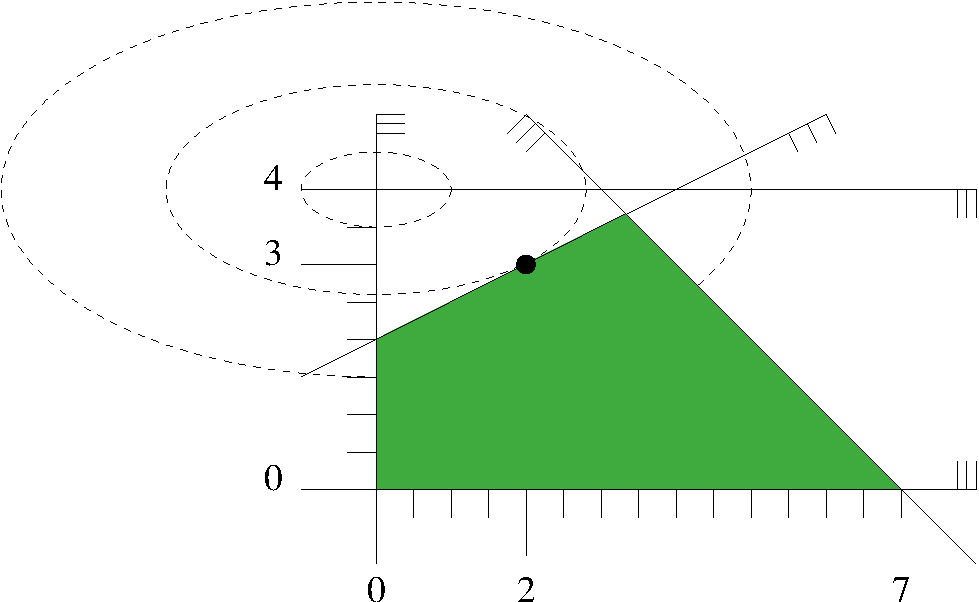
\includegraphics{QP_solver/first_qp} % omit suffix .eps to supprt PS and PDF
\end{center}
\end{ccTexOnly}

\begin{ccHtmlOnly}
<CENTER>
<IMG BORDER=0 SRC="./first_qp.png" ALIGN=middle ALT="A quadratic program in two variables">
</CENTER>
\end{ccHtmlOnly}

\caption{A quadratic program in two variables
\label{fig:QP-first_qp}}
\end{figure}

\subsection{Constructing a program from data}
Here is how this quadratic program can be solved in \cgal\ 
according to the first way (letting the model take care of
the data). We use \ccc{int} as the entry type, and 
\ccc{MP_Float} or \ccc{Gmpz} (which is faster and preferrable if
\texttt{GMP} is installed) as the exact type for the
internal computations. For examples 
how to work with the input type \ccc{double}, we refer to 
Sections \ref{sec:QP-iterators} and \ref{sec:QP-customization}.

{\bf Note:} For the quadratic objective function, the entries 
of the matrix $2D$ have to be provided, rather than $D$. Although 
this is common to almost all quadratic programming solvers, it 
can easily be overlooked by a novice.

\ccIncludeExampleCode{QP_solver/first_qp.cpp}

The output of the above program is:
\begin{verbatim}
status:          OPTIMAL
objective value: 8/1
variable values:
  0: 2/1
  1: 3/1
\end{verbatim}

\subsection{Constructing a program from a stream}
Here, the program data must be available in \ccc{MPSFormat} (the
\ccc{MPSFormat} page shows how our running example looks like in
this format, and it briefly explains the format). Assuming that
your working directory contains the file \texttt{first\_qp.mps},
the following program will read and solve it, with the same output
as before.

\ccIncludeExampleCode{QP_solver/first_qp_from_mps.cpp}

\subsection{Constructing a program from iterators}
The following program again solves our running example from above,
with the same output, but this time with iterators over data stored 
in suitable containers. You can see that we also store zero 
entries here (in $D$). For this toy problem, the previous two
approaches (program from data/stream) are clearly preferrable, 
but Section \ref{sec:QP-iterators} shows an
example where it makes sense to use the iterator-based approach.

\ccIncludeExampleCode{QP_solver/first_qp_from_iterators.cpp}

{\bf Note 1:} The example shows an interesting feature of this approach:
not all data need to come from containers. Here, the iterator over the
vector of relations can be provided through the class
\ccc{Const_oneset_iterator<T>}, since all entries of this vector
are equal to \ccc{CGAL::SMALLER}. The same could have been done with
the vector \ccc{fl} for the finiteness of the lower bounds. 

{\bf Note 2:} The program type looks a bit scary, with its total of
9 template arguments, one for each iterator type. In Section
\ref{sec:QP-makers} we show how the explicit construction of
this type can be circumvented.

\section{Solving Linear and Nonnegative Programs\label{sec:QP-lp}}
Let us reconsider the general form of (QP) from Section \ref{sec:QP-def} 
above. If $D=0$, the quadratic program is in fact a \emph{linear program},
and in the case that the bound vectors $l$ is the zero vector and all 
entries of $u$ are $\infty$, the program is said to be \emph{nonnegative}. 
The package offers dedicated models and solution methods for these special
cases.

From an interface perspective, this is just syntactic sugar: in the 
model \ccc{Quadratic_program<NT>}, we can easily set the default bounds 
so that a nonnegative program results, and a linear program is
obtained by simply not inserting any $D$-entries. Even in the
iterator-based approach (see 
\ccReferToExampleCode{QP_solver/first_qp_from_iterators.cpp}), linear
and nonnegative programs can easily be defined through suitable 
\ccc{Const_oneset_iterator<T>}-style iterators.

The main reason for having dedicated solution methods for linear and
nonnegative programs is efficiency: if the solver knows that the program
is linear, it can save some computations compared to the general solver
that unknowingly has to fiddle around with a zero $D$-matrix. As in
Section \ref{sec:QP-robustness} above, we can argue that checking in
advance whether $D=0$ is not an option in general, since this may require 
$\Omega(n^2)$ time on the dense interface.

Similarly, if the solver knows that the program is nonnegative, it
will be more efficient than under the general bounds 
$\qpl\leq \qpx \leq \qpu$.
You can argue that nonnegativity \emph{is} something that could easily
be checked in time $O(n)$ beforehand, but then again nonnegative
programs are so frequent that the syntactic sugar aspect becomes
somewhat important. After all, we can save four iterators in 
specifying a nonnegative linear program in terms of the concept 
\ccc{NonnegativeLinearProgram} rather than 
\ccc{LinearProgram}.

Often, there are no bounds at all for the variables, i.e., all entries
of $\qpl$ are $-\infty$, and all entries of $\qpu$ 
are $\infty$ (this is
called a \emph{free} program). There is no dedicated solution method
for this case (a free quadratic or linear program is treated like a
general quadratic or linear program), but all predefined models make
it easy to specify all sorts of default bounds, covering the free 
case.

\subsection{The linear programming solver}
Let's go back to our first quadratic program from above and change it 
into a linear program by simply removing the quadratic part of the
objective function:

\[
\begin{array}{lrcl}
\mbox{minimize}       & - 32y + 64 \\
\mbox{subject to}     & x + y &\leq& 7 \\
                      & -x + 2y &\leq& 4 \\
                      & x &\geq& 0 \\
                      & y &\geq& 0 \\
                      & y &\leq& 4
\end{array}
\] 

Figure \ref{fig:QP-first_lp} shows how this looks like. We will not
visualize a linear objective function with contour lines but with
arrows instead. The arrow represents the (direction) of the vector $-c$,
and we are looking for a feasible solution that is ``extreme'' in the direction
of the arrow. In our small example, this is the unique point ``on'' the
two constraints $x_1+x_2\leq 7$ and $-x_1+x_2\leq 4$, the point
$(10/3,11/3)$ marked with a black dot. The optimal objective function
value is $-32(11/3)+64=-160/3$.

\begin{figure}[htbp]
\begin{ccTexOnly}
\begin{center}
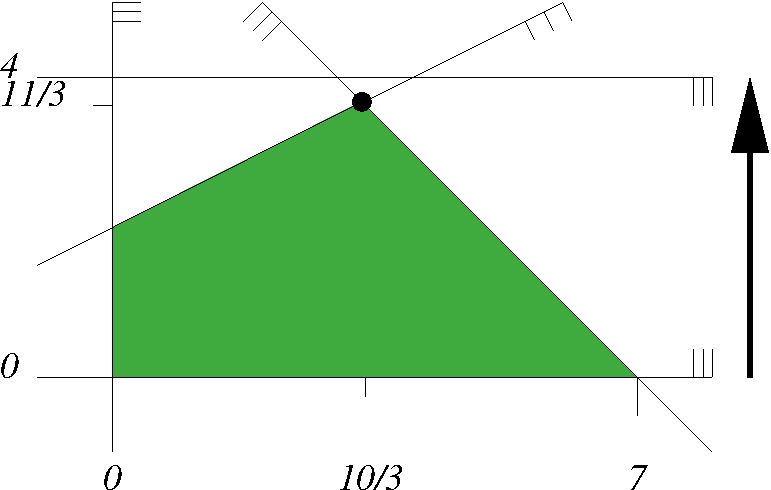
\includegraphics{QP_solver/first_lp} % omit suffix .eps to supprt PS and PDF
\end{center}
\end{ccTexOnly}

\begin{ccHtmlOnly}
<CENTER>
<IMG BORDER=0 SRC="./first_lp.png" ALIGN=middle ALT="A linear program in two variables">
</CENTER>
\end{ccHtmlOnly}

\caption{A linear program in two variables
\label{fig:QP-first_lp}}
\end{figure}

Here is \cgal\ code for solving it, using the dedicated LP solver, and
according to the three ways for constructing a program that we have
already discussed in Section \ref{sec:QP-first}. 

\ccReferToExampleCode{QP_solver/first_lp.cpp}\\
\ccReferToExampleCode{QP_solver/first_lp_from_mps.cpp}\\
\ccReferToExampleCode{QP_solver/first_lp_from_iterators.cpp}

In all cases, the output is
\begin{verbatim}
status:          OPTIMAL
objective value: -160/3
variable values:
  0: 10/3
  1: 11/3
\end{verbatim}

\subsection{The  nonnegative quadratic programming solver}
If we go back to our first quadratic program and
remove the constraint $y\leq 4$, we arrive at a nonnegative quadratic
program: 

\[
\begin{array}{lrcl}
\mbox{minimize}       & x^2 + 4(y-4)^2 &(=& x^2 + 4y^2 - 32y + 64) \\
\mbox{subject to}     & x + y &\leq& 7 \\
                      & -x + 2y &\leq& 4 \\
                      & x,y &\geq& 0
\end{array}
\]

Figure \ref{fig:QP-first_nonnegative_qp} contains 
the illustration; since the constraint $y\leq 4$ was 
redundant, the feasible region and the optimal solution do 
not change. 

\begin{figure}[htbp]
\begin{ccTexOnly}
\begin{center}
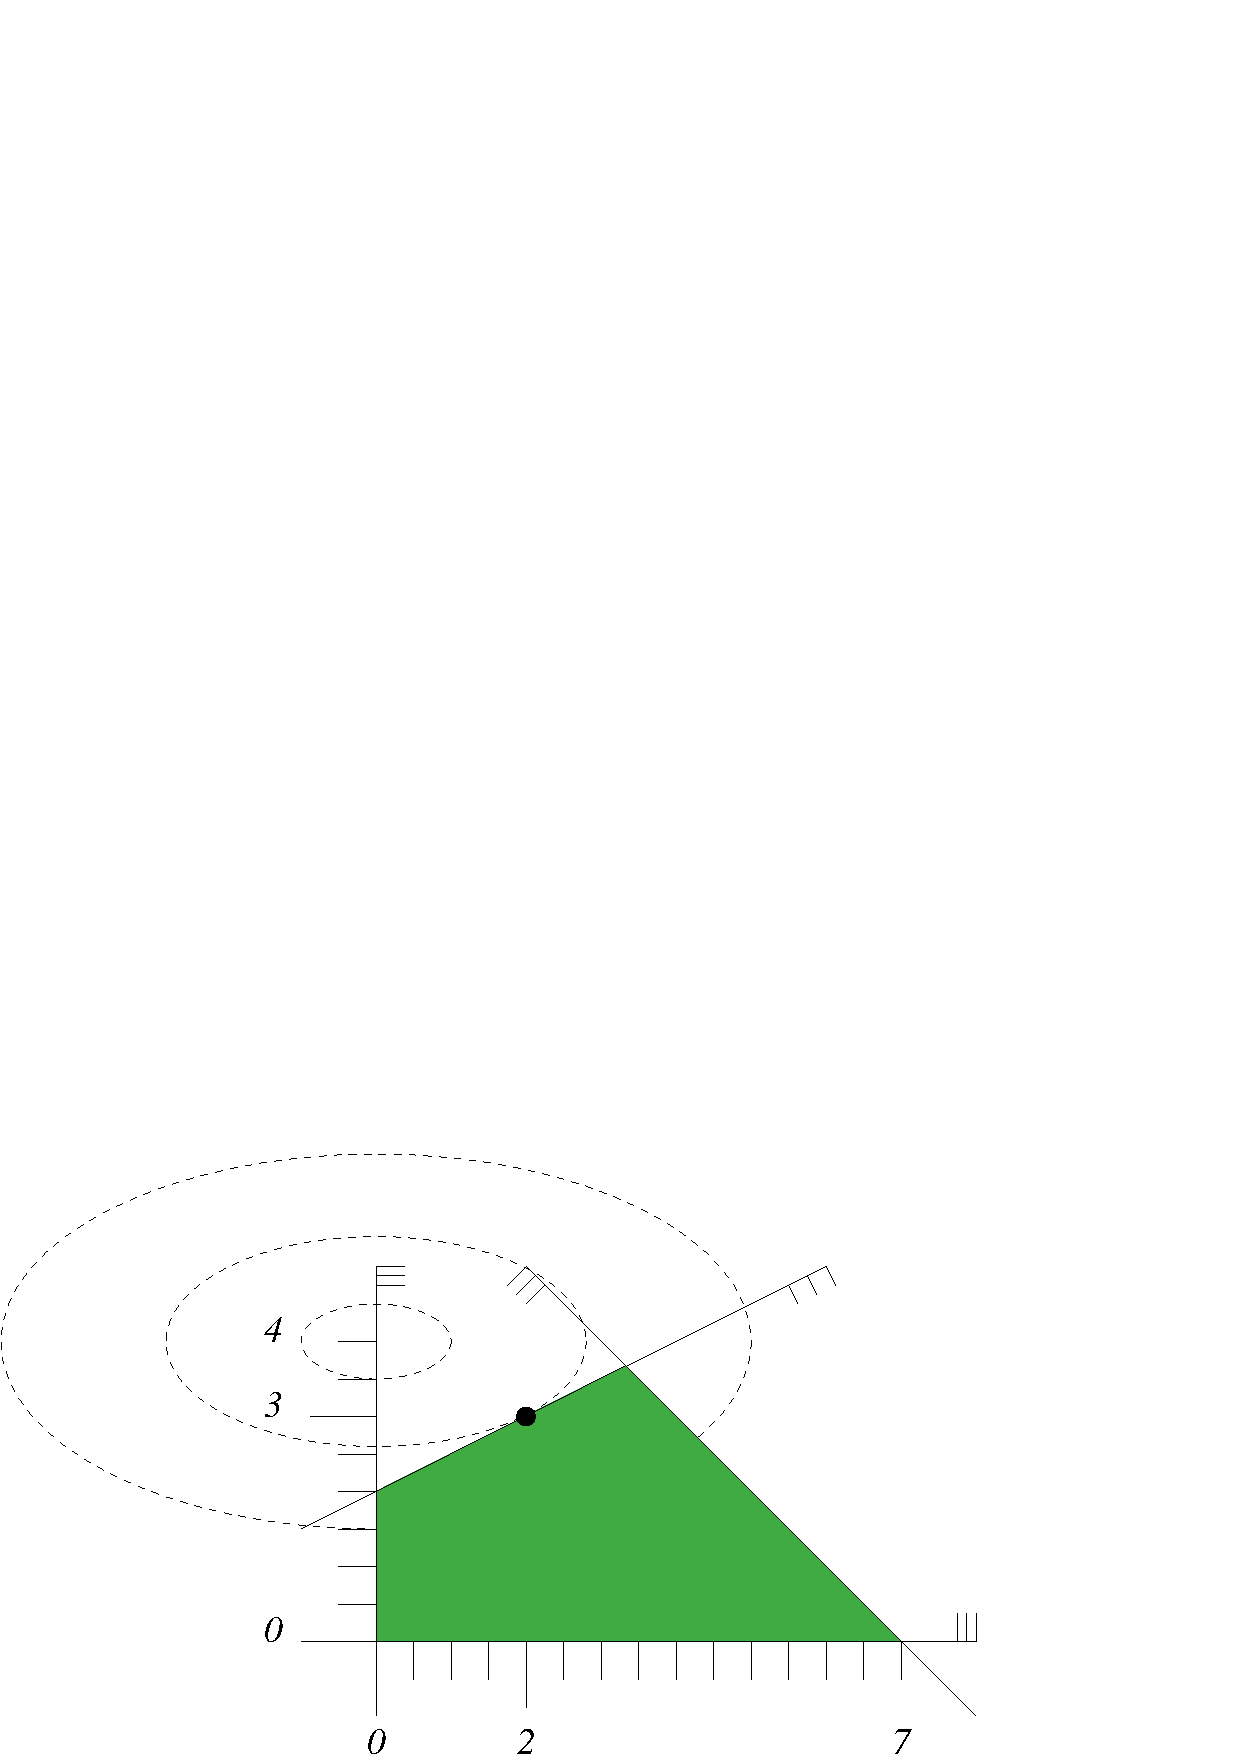
\includegraphics{QP_solver/first_nonnegative_qp} 
\end{center}
\end{ccTexOnly}

\begin{ccHtmlOnly}
<CENTER>
<IMG BORDER=0 SRC="./first_nonnegative_qp.png" ALIGN=middle ALT="A linear program in two variables">
</CENTER>
\end{ccHtmlOnly}

\caption{A nonnegative quadratic program in two variables
\label{fig:QP-first_nonnegative_qp}}
\end{figure}

The following programs (using the dedicated solver for nonnegative
quadratic programs) will therefore again output
\begin{verbatim}
status:          OPTIMAL
objective value: 8/1
variable values:
  0: 2/1
  1: 3/1
\end{verbatim}

\ccReferToExampleCode{QP_solver/first_nonnegative_qp.cpp}\\
\ccReferToExampleCode{QP_solver/first_nonnegative_qp_from_mps.cpp}\\
\ccReferToExampleCode{QP_solver/first_nonnegative_qp_from_iterators.cpp}

\subsection{The nonnegative linear programming solver}
Finally, a dedicated model and function is available for nonnnegative linear
programs as well. Let's take our linear program from above and remove
the constraint $y\leq 4$ to obtain a nonnegative linear program. At
the same time we remove the constant objective function term to get
a ``minimal'' input and a ``shortest'' program; the optimal value is
$-32(11/3)=-352/3$.

\[
\begin{array}{lrcl}
\mbox{minimize}       & - 32y \\
\mbox{subject to}     & x + y &\leq& 7 \\
                      & -x + 2y &\leq& 4 \\
                      & x,y &\geq& 0 \\
\end{array}
\] 

This can be solved by any of the following three programs

\ccReferToExampleCode{QP_solver/first_nonnegative_lp.cpp}\\
\ccReferToExampleCode{QP_solver/first_nonnegative_lp_from_mps.cpp}\\
\ccReferToExampleCode{QP_solver/first_nonnegative_lp_from_iterators.cpp}

The output will always be
\begin{verbatim}
status:          OPTIMAL
objective value: -352/3
variable values:
  0: 10/3
  1: 11/3
\end{verbatim}

\section{Working from Iterators\label{sec:QP-iterators}}
Here we present a somewhat more advanced example that emphasizes the
usefulness of solving linear and quadratic programs from iterators. 
Let's look at a situation in which a linear program is given implicitly, 
and access to it is gained through properly constructed iterators.

The problem we are going to solve is the following: given points
$p_1,\ldots p_{n}$ in $d$-dimensional space and another point $p$: is
$p$ in the convex hull of $\{p_1,\ldots,p_{n}\}$? In formulas, this is
the case if and only if there are real coefficients
$\lambda_1,\ldots,\lambda_n$ such that $p$ is a convex combination of
$p_1,\ldots,p_n$: 
\[
p = \sum_{j=1}^{n}~\lambda_j~p_j, \quad \sum_{j=1}^{n}~\lambda_j = 1,
\quad \lambda_j \geq 0 \mbox{~for all $j$.}
\]
The problem of testing the existence of such $\lambda_j$ can 
be expressed as a linear program. It becomes particularly easy
when we use the homogeneous representations of the points: if
$q_1,\ldots,q_n,q\in\R^{d+1}$ are homogeneous coordinates for
$p_1,\ldots,p_n,p$ with positive homogenizing coordinates 
$h_1,\ldots,h_n,h$, we have
\[q_j = h_j \cdot (p_j \mid 1) \mbox{~for all $j$, and~} q = h \cdot
(p\mid 1).\] Now, nonnegative $\lambda_1,\ldots,\lambda_n$ are
suitable coefficients for a convex combination if and only if
\[\sum_{j=1}^n~ \lambda_j(p_j \mid 1) = (p\mid 1), \]
equivalently, if there are $\mu_1,\ldots,\mu_n$ 
(with $\mu_j = \lambda_j \cdot h/{h_j}$ for all $j$) such that
\[
\sum_{j=1}^n~\mu_j~q_j = q, \quad \mu_j \geq 0\mbox{~for all $j$}.
\]

The linear program now tests for the existence of nonnegative $\mu_j$
that satisfy the latter equation. Below is the code; it defines a
function that solves the linear program, given $p$ and
$p_1,\ldots,p_n$ (through an iterator range). The only (mild)
trickery involved is the construction of the nested iterator 
through a fixed column of the constraint matrix $A$. We get this
from transforming the iterator through the points using a functor 
that maps a point to an iterator through its homogeneous coordinates.

\ccIncludeExampleCode{QP_solver/solve_convex_hull_containment_lp.h}

To see this in action, let us call it with $p_1=(0,0), p_2=(10,0),
p_3=(0,10)$ fixed (they define a triangle) and all integral points $p$
in $[0,10]^2$. We know that $p$ is in the convex hull of
$\{p_1,p_2,p_3\}$ if and only if its two coordinates sum up to $10$ at
most. As the exact type, we use \ccc{MP_Float}.

\ccIncludeExampleCode{QP_solver/convex_hull_containment.cpp}

\subsection{Using makers\label{sec:QP-makers}}
You already noticed in the previous example that the actual 
template arguments for 
\ccc{CGAL::Nonnegative_linear_program_from_iterators<A_it, B_it, R_it, C_it>} 
can be quite elaborate, and this only gets worse if you plug more 
iterators into each other. In general, you want to construct a 
program from given expressions for the iterators, but the
types of these expressions are probably very complicated and 
difficult to look up. 

You can avoid the explicit construction of the type
\ccc{CGAL::Nonnegative_linear_program_from_iterators<A_it, B_it, R_it, C_it>} 
if you only need an expression of it, e.g.\ to pass it directly 
as an argument to the solving function. Here is an alternative
version of 
\ccReferToExampleCode{QP_solver/solve_convex_hull_containment_lp.h}
that shows how this works. In effect, you get shorter and more
readable code.

\ccIncludeExampleCode{QP_solver/solve_convex_hull_containment_lp2.h}


\section{Important Variables and Constraints}
If you have a solution $\qpx^*$ of a linear or quadratic program,
the ``important'' variables are typically the ones that are not on
their bounds. In case of a nonnegative program, these are the nonzero
variables.  Going back to the example of the previous Section
\ref{sec:QP-iterators}, we can easily interpret their
importance: the nonzero variables correspond to points $p_j$ that
actually contribute to the convex combination that yields $p$. 

The following example shows how we can access the important variables,
using the iterators \ccc{basic_variable_indices_begin()} and
\ccc{basic_variable_indices_end()}.

We generate a set of points that form a 4-gon in $[0,4]^2$, and then find 
the ones that contribute to the convex combinations of all 25 lattice 
points in $[0,4]^2$. If the lattice point in question is not in the 4-gon, 
we simply output this fact. 

\ccIncludeExampleCode{QP_solver/important_variables.cpp}

It turns out that exactly three of the four points contribute to any
convex combination, even through there are lattice points that lie
in the convex hull of less than three of the points. This shows that
the set of basic variables that we access in the example does not
necessarily coincide with the set of important variables as defined
above. In fact, it is only guaranteed that a non-basic variable 
attains one of its bounds, but there might be basic variables that
also have this property. In linear and quadratic programming terms,
such a situation is called a \emph{degeneracy}.

There is also the concept of an important constraint: this is 
typically a constraint in the system $A\qpx\qprel\qpb$ 
that is satisfied with equality at $\qpx^*$. Program
\ccReferToExampleCode{QP_solver/first_qp_basic_constraints.cpp}
shows how these can be accessed, using the iterators
\ccc{basic_constraint_indices_begin()} and
\ccc{basic_constraint_indices_end()}.

Again, we have a disagreement
between ``basic'' and ``important'': it is guaranteed that all
basic constraints are satisfied with equality at $\qpx^*$, but there 
might be non-basic constraints that are satisfied with equality
as well.

\section{Solution Certificates\label{sec:QP-certificates}}
Suppose the solver tells you that the problem you have entered is
infeasible. Why should you believe this? Similarly, you can
quite easily verify that a claimed optimal solution is feasible,
but why is there no better one? 

Certificates are proofs that the solver can give you in order
to convince you that what it claims is indeed true. The archetype 
of such a proof is \emph{Farkas Lemma} \cite{cgal:mg-uulp-06}.

{\bf Farkas Lemma:} \emph{Either} the inequality system
\[
\begin{array}{rcl}
A \qpx & \leq & \qpb \\
  \qpx & \geq & 0
\end{array}
\]
has a solution $\qpx^*$, \emph{or} there exists a vector $\qpy$ such
that
\[
\begin{array}{rcl}
   \qpy &\geq& 0\\ 
\qpy^TA &\geq& 0\\ 
\qpy^T\qpb & < &  0,
\end{array}
\]
but not both.

Thus, if someone wants to convince you that the first system in
the Farkas Lemma is infeasible, that person can simply give you
a vector $\qpy$ that solves the second system. Since you can easily
verify yourself that the $\qpy$ you got satisfies this second system, 
you now have a certificate for the infeasibility of the first system,
assuming that you believe in Farkas Lemma. 

Here we show how the solver can convince you. We first set up an infeasible
linear program with constraints of the type $A\qpx\leq \qpb, \qpx\geq 0$; then
we solve it and ask for a certificate. Finally, we verify the certificate
by simply checking the inequalities of the second system in Farkas
Lemma.

\ccIncludeExampleCode{QP_solver/infeasibility_certificate.cpp}

There are similar certificates for optimality and unboundedness
that you can see in action in the programs
\ccReferToExampleCode{QP_solver/optimality_certificate.cpp} and
\ccReferToExampleCode{QP_solver/unboundedness_certificate.cpp}.
The underlying variants of Farkas Lemma are somewhat more
complicated, due to the mixed relations in $\qprel$ and the general
bounds. The certificate section of \ccc{Quadratic_program_solution<ET>} 
gives the full picture and mathematically proves the correctness
of the certificates.

\section{Customizing the Solver\label{sec:QP-customization}}
Sometimes it is necessary to alter the default behavior of the solver.
There are two notable case that we want to discuss here. There are
other situations where such changes are not critical but simply beneficial
for the performance (see the class \ccc{Quadratic_program_pricing_strategy}
for a discussion).

\subsection{Exponent overflow in double using floating-point filters\label{sec:QP-customization-filtering}}
The filtered version of the solver that is used by default on input
type \ccc{double} internally constructs double-approximations of exact
multiprecision values. If these exact values are extremely large, this
may lead to \emph{infinite} \ccc{double} values and incorrect results.
In debug mode, the solver will notice this through a certificate 
cross-check in the end (or even earlier). In this case, it is advisable
to switch to a non-filtered \emph{pricing strategy}, see
\ccc{Quadratic_program_pricing_strategy}.

Consider the following program. It reads a nonnegative linear program from
the file \texttt{filter\_failure.mps} (which is in the example directory as 
well), and then solves it using \emph{Dantzig's rule}.

\ccIncludeExampleCode{QP_solver/filter_failure.cpp}

If your comment the line
\begin{verbatim}
options.set_pricing_strategy(CGAL::QP_DANTZIG);        // Dantzig's rule
\end{verbatim}
you will see that the solver fails (in debug mode, it will run into
an assertion, and in non-debug mode, the objective value is simply 
wrong). This is due to a filture failure, and switching to a non-filtered
variant like \ccc{QP_DANTZIG} solves the problem.

\subsection{The solver internally cycles\label{sec:QP-customization-cycling}}
Consider the following program. It reads a nonnegative linear program from 
the file \texttt{cycling.mps} (which is in the example directory as well),
and then solves it in verbose mode, using \emph{Bland's rule}, see
\ccc{Quadratic_program_pricing_strategy}.

\ccIncludeExampleCode{QP_solver/cycling.cpp}

If you comment the line 
\begin{verbatim}
options.set_pricing_strategy(CGAL::QP_BLAND);          // Bland's rule
\end{verbatim}
you will see that the solver cycles: the verbose mode outputs the same
sequence of six iterations over and over again. By switching to 
\ccc{QP_BLAND}, the solution process typically slows down a bit 
(it may also speed up in some cases), but now it is guaranteed that
no cycling occurs.

In general, the verbose mode can be of use when you are not sure whether 
the solver ``has died'', or whether it simply takes very long to solve
your problem.  We refer to the class \ccc{Quadratic_program_options}
for further details.

\section{Some Benchmarks\label{sec:QP-benchmark}}
Here we want to show what you can expect from the solver's performance
in a specific application; we don't know whether this application is 
typical in your case, and we make no claims whatsoever about the 
performance in other applications.

Still, the example shows that the performance can be dramatically 
affected by switching between pricing strategies, and this message
is important to know if you want to achieve good performance in 
general. 

The application is the one already discussed in Section \ref{sec:QP-iterators}
above: testing whether a point is in the convex hull of other points.
To be able to switch between pricing strategies, we add another
parameter of type \ccc{Quadratic_program_options} to the function
\ccc{solve_convex_hull_containment_lp} that we pass on to the solution
function:

\ccIncludeExampleCode{QP_solver/solve_convex_hull_containment_lp3.h}

Now let us test containment of the origin in the convex hull
of $n$ random points in $[0,1]^d$ (it will most likely not be contained,
and it turns out that this is the most expensive case). In the program
below, we use $d=10$ and $n=100,000$, and we comment on some other
combinations of $n$ and $d$ below (feel free to experiment with still other
values).

\ccIncludeExampleCode{QP_solver/convex_hull_containment_benchmarks.cpp}

If you compile with the macros \texttt{NDEBUG} or
\texttt{CGAL\_QP\_NO\_ASSERTIONS} set (this is essential for good
performance!!), you will see runtimes that qualitatively look as
follows (on your machine, the actual runtimes will roughly be some
fixed multiples of the numbers in the table below). The default
choice of the pricing strategy in that case is 
\ccc{QP_PARTIAL_FILTERED_DANTZIG}.

\begin{tabular}{lcl}
strategy & &runtime in seconds \\ \hline
\ccc{CGAL::QP_CHOOSE_DEFAULT} & | &  0.32\\
\ccc{CGAL::QP_DANTZIG}     & | &    10.7    \\      
\ccc{CGAL::QP_PARTIAL_DANTZIG}  & | &  3.72  \\     
\ccc{CGAL::QP_BLAND}  & | &            3.65  \\
\ccc{CGAL::QP_FILTERED_DANTZIG}   & | &  0.43  \\  
\ccc{CGAL::QP_PARTIAL_FILTERED_DANTZIG}& | & 0.32
\end{tabular}

We clearly see the effect of filtering: we gain a factor of ten,
roughly, compared to the next best non-filtered variant. 

\subsection{$d=3$, $n=1,000,000$} 
The filtering effect is amplified if the points/dimension ratio becomes
larger. This is what you might see in dimension three, with one million
points. 

\begin{tabular}{lcl}
strategy & &runtime in seconds \\ \hline
\ccc{CGAL::QP_CHOOSE_DEFAULT} & | & 1.34 \\
\ccc{CGAL::QP_DANTZIG}     & | &    47.6   \\      
\ccc{CGAL::QP_PARTIAL_DANTZIG}  & | &  15.6  \\     
\ccc{CGAL::QP_BLAND}  & | &            16.02  \\
\ccc{CGAL::QP_FILTERED_DANTZIG}   & | &  1.89  \\  
\ccc{CGAL::QP_PARTIAL_FILTERED_DANTZIG}& | & 1.34
\end{tabular}

\subsection{$d=100$, $n=100,000$}
Increasing the dimension to $100$ compared to the above example clearly
shows that the filtering effect deteriorates with higher dimension but
is still noticeable.

\begin{tabular}{lcl}
strategy & &runtime in seconds \\ \hline
\ccc{CGAL::QP_CHOOSE_DEFAULT} & | & 3.05 \\
\ccc{CGAL::QP_DANTZIG}     & | &    78.4   \\      
\ccc{CGAL::QP_PARTIAL_DANTZIG}  & | &  45.9  \\     
\ccc{CGAL::QP_BLAND}  & | &            33.2  \\
\ccc{CGAL::QP_FILTERED_DANTZIG}   & | &  3.36  \\  
\ccc{CGAL::QP_PARTIAL_FILTERED_DANTZIG}& | & 3.06
\end{tabular}

\subsection{$d=500$, $n=1,000$} 
If the points/dimension ratio tends to a constant, filtering is no
longer a clear winner. The reason is that the numbers involved in the
necessary exact calculations are so large that the overall performance is
dominated by them.

\begin{tabular}{lcl}
strategy & &runtime in seconds \\ \hline
\ccc{CGAL::QP_CHOOSE_DEFAULT} & | & 2.65 \\
\ccc{CGAL::QP_DANTZIG}     & | &  5.55     \\      
\ccc{CGAL::QP_PARTIAL_DANTZIG}  & | & 5.6   \\     
\ccc{CGAL::QP_BLAND}  & | &       4.46       \\
\ccc{CGAL::QP_FILTERED_DANTZIG}   & | &  2.65  \\  
\ccc{CGAL::QP_PARTIAL_FILTERED_DANTZIG}& | & 2.61
\end{tabular}
